\documentclass[dvipsnames]{article}
\usepackage{marvosym}

%...TikZ & PGF
\usepackage{pgfplots}
\pgfplotsset{compat=1.11}
\tikzset{>=latex}
\usetikzlibrary{calc,math}
\usepackage{tikzsymbols}
\usepgfplotslibrary{fillbetween}
\usetikzlibrary{decorations.markings} 
\usetikzlibrary{arrows.meta} %...APP2 for arrows as objects and images
\usetikzlibrary{backgrounds} %...For shading portions of graphs
\usetikzlibrary{patterns} %...Unit 5 Problems
\usetikzlibrary{shapes.geometric} %...For drawing cylinders in Unit 2
\usepackage{makecell} %...use \thead{} to enable line skip in table headers
\tikzset{
    mark position/.style args={#1(#2)}{
        postaction={
            decorate,
            decoration={
                markings,
                mark=at position #1 with \coordinate (#2);
            }
        }
    }
} %...See https://tex.stackexchange.com/questions/43960/define-node-at-relative-coordinates-of-draw-plot

\tikzset{
    declare function = {trajectoryequation10(\x,\vi,\thetai)= tan(\thetai)*\x - 10*\x^2/(2*(\vi*cos(\thetai))^2);},
    declare function = {trajectoryequation(\x,\vi,\thetai)= tan(\thetai)*\x - 9.8*\x^2/(2*(\vi*cos(\thetai))^2);},
    declare function = {patheq(\x,\yi,\vi,\thetai)= \yi + tan(\thetai)*\x - 9.8*\x^2/(2*(\vi*cos(\thetai))^2);},
    declare function = {patheqten(\x,\yi,\vi,\thetai)= \yi + tan(\thetai)*\x - 10*\x^2/(2*(\vi*cos(\thetai))^2);} %like patheq but with gravity = 10
}

%...siunitx
\usepackage{siunitx}
\DeclareSIUnit{\nothing}{\relax}
\def\mymu{\SI{}{\micro\nothing} }
\DeclareSIUnit\mmHg{mmHg}
\DeclareSIUnit{\mile}{mi}
%...NOTE: "The product symbol between the number and unit is set using the quantity-product option."

%...Other
\usepackage{amsthm}
\usepackage{amsmath}
\usepackage{amssymb}
\usepackage{cancel}
\usepackage{subcaption}
\usepackage{dashrule}
\usepackage{enumitem}
\usepackage{fontawesome}
\usepackage{multicol}
\usepackage{glossaries}
%\numberwithin{equation}{section}
\numberwithin{figure}{section}
\usepackage{float}
\usepackage{twemojis} %...twitter emojis
\usepackage{utfsym}
\usepackage{linearb} %...For \BPwheel in Unit 8
\newcommand{\R}{\mathbb{R}} %...real number symbol
\usepackage{graphicx}
\graphicspath{ {../Figures/} }
\usepackage{hyperref}
\hypersetup{colorlinks=true,
    linkcolor=blue,
    filecolor=magenta,
    urlcolor=cyan,}
\urlstyle{same}
\newcommand{\hdashline}{{\hdashrule{\textwidth}{0.5pt}{0.8mm}}}
\newcommand{\hgraydashline}{{\color{lightgray} \hdashrule{0.99\textwidth}{1pt}{0.8mm}}}

%...Miscellaneous user-defined symbols
\newcommand{\fnet}{F_{\text{net}}} %...For net force
\newcommand{\bvec}[1]{\vec{\mathbf{#1}}} %...bold vector
\newcommand{\bhat}[1]{\,\hat{\mathbf{#1}}} %...bold hat vector
\newcommand{\que}{\mathord{?}}  %...Question mark symbol in equation env
%...Define thick horizontal rule for examples:
\newcommand{\hhrule}{\hrule\hrule}
\let\oldtexttt\texttt% Store \texttt
\renewcommand{\texttt}[2][black]{\textcolor{#1}{\ttfamily #2}}% 

%...For use in the exam document class
\newif\ifprintmetasolutions


%...Decreases space above and below align and gather enironment
\makeatletter
\g@addto@macro\normalsize{%
  \setlength\abovedisplayskip{-3pt}
  \setlength\belowdisplayskip{6pt} 
}
\makeatother





\usepackage[margin=1in]{geometry}
\usepackage{OutilsGeomTikz}

%...Theorem for examples
\theoremstyle{definition}
\newtheorem{example}{Example}
\newtheorem{exercise}{Exercise}

%...Define colors for use in Unit 11: SHM and Waves
\pgfdeclarehorizontalshading{visiblelight}{50bp}{
color(0.00000000000000bp)=(red);
color(8.33333333333333bp)=(orange);
color(16.66666666666670bp)=(yellow);
color(25.00000000000000bp)=(green);
color(33.33333333333330bp)=(cyan);
color(41.66666666666670bp)=(blue);
color(50.00000000000000bp)=(violet)
}

\setlength\parindent{0pt}
\setlength{\parskip}{6pt}

\renewcommand{\thesubsubsection}{\thesubsection\alph{subsubsection}}


\usepackage{circuitikz}
\begin{document}






\subsection*{\ref{DicxAf} Exercises}



\subsection{Transfer of Electric Charge} \label{XFJNUr}



\hrule

\begin{multicols}{2}

\subsection*{\ref{XFJNUr} Exercises}

\textbf{\ref{IyrMKh}--\ref{VKqxLG}} Do a Google search for the \href{https://phet.colorado.edu/en/simulations/balloons-and-static-electricity/about}{PhET Simulation} called \texttt{Balloons and Static Electricity}. Rub 1 balloon against the shirt. Observe how it can stick to the shirt and to the wall. Click \texttt{Reset Balloon}.
Next, rub 1 balloon against one half of the shirt, and the other balloon against the other half of the shirt. Observe how the balloons are attracted to the shirt but repelled by each other.

\begin{exercise} \label{IyrMKh}
    What happens to the electrons ($-$) when you rub the shirt against the balloon?
\end{exercise}

\begin{exercise}
    What does it mean that a balloon has an ``electron excess''?
\end{exercise}

\begin{exercise}
    What does it mean that the wool shirt has an ``electron deficit'?
\end{exercise}

\begin{exercise}
    Why is the balloon attracted to the shirt?
\end{exercise}

\begin{exercise} \label{VKqxLG}
    Why are the balloons repelled by each other?
\end{exercise}

\hrule

\begin{exercise} \label{9U7zJj}
    Look at Equation (\ref{Dabfyz}) for the charge on an object that has an electron excess. What equation would you use to calculate the net charge on an object that has an electron \textit{deficit}?
\end{exercise}

\begin{exercise} \label{gEsEJ7}
    A rain cloud discharges 5 billion billion excess electrons through a lightning strike. What is the total charge carried by the lightning strike?
\end{exercise}



\begin{exercise} \label{d3zygU}
    What is the charge on a dust particle that contains five thousand excess electrons?
\end{exercise}

\begin{exercise} \label{ERkfIH}
    If an electric fence delivers \SI{4.2e16}{} electrons to a person who touches it, what is the electric charge transferred to the person?
\end{exercise}

\begin{exercise} \label{9qwZGy}
    How many protons are required to make \SI{2.89}{C} of charge?
\end{exercise}

\end{multicols}

\hrule

\subsection{Powers of 10} \label{tdVujC}

Powers of 10 and scientific notation are powerful ways to write very large and very small numbers. Powers of 10 work as follows:

\begin{equation*}
    10^0 = 1\ , \quad 10^1 = 10\ , \quad 10^2 = 100\ , \quad 10^3 = \SI{1000}{}\ , \qquad 10^6 = \SI{1000000}{}\ \qquad 10^{11} = \SI{100000000000}{}
\end{equation*}

Likewise,

\begin{equation*}
    10^{-1} = \frac{1}{10} = 0.1\ , \quad
    10^{-2} = \frac{1}{100} = \SI{0.01}{}\ , \quad 
    10^{-5} = \frac{1}{\SI{100000}{}} = 0.000\,01\ ,\qquad
    10^{-8} = \frac{1}{\num{100000000}} = 0.000\,000\,01
\end{equation*}

In this unit, when working with scientific notation and powers of ten, we will often be dividing powers of 10. For example, $10^2/10^{-3}$. Here we may apply the following quotient property.


\begin{example}
    Calculate $10^7/10^4$ by hand.
\end{example}

Solution: This fraction is worked out as follows:

\begin{equation*}
    \frac{10^7}{10^4} = 10^{7-4} = 10^3
\end{equation*}

\begin{example}
    Calculate $10^2/10^{-3}$ by hand.
\end{example}

Solution: The solution is

\begin{equation*}
    \frac{10^2}{10^{-3}} = 10^{2 - (-3)} = 10^5
\end{equation*}

\hrule
\vspace{1em}

The following property reminds us how to compute such fractions generally.

\begin{center}
    \textbf{Quotient Property for Exponents.} If $m$ and $n$ are integers, then

    \begin{equation} \label{6Kyqsn}
        \frac{10^m}{10^n} = 10^{m-n}
    \end{equation}
\end{center}




\begin{example}
    The net charge on a microscopic piece of silver is \SI{-5}{nC}. (a) What does the silver piece have: electron excess or electron deficit? (b) How many electrons are in excess/deficit compared to neutrality?
\end{example}

Solution: (a) Since the silver's charge is negative, it must have excess electrons (more electrons than protons).

\vspace{1em}

(b) The metric prefix nC means \textit{nano}coulomb, where \textit{nano} represents $10^{-9}$. Therefore, the net charge is $q = \SI{-5}{nC} = \SI{-5e-9}{C}$. As usual, the elementary charge is $e= \SI{1.602e-19}{C}$. By Equation (\ref{Dabfyz}),

\begin{equation*}
    q = -ne
\end{equation*}

Substituting known values, while omitting units, leads to

\begin{equation*}
     \num{-5e-9} = - n\,(\num{1.602e-19})
\end{equation*}

We solve this equation for the number of electrons as follows:

\begin{align*}
    \textbf{Write $n$ on left} \qquad & - n\,(\SI{1.602e-19}{}) = \SI{-5e-9}{}\\[1ex]
    \textbf{Divide by \SI{-1.602e-19}{}} \qquad & \frac{- n\,(\cancel{\SI{1.602e-19}{}})}{- \textcolor{red}{\cancel{\SI{1.602e-19}{}}}} = \frac{\SI{-5e-9}{}}{- \textcolor{red}{\SI{1.602e-19}{}}}\\[1ex]
    \textbf{Simplify} \qquad & n = \frac{\qty{5e-9}{}}{\qty{1.602e-19}{}}\\[1ex]
    \textbf{Separate factors} \qquad & \frac{5}{1.602} \times \frac{10^{-9}}{10^{-19}}\\[1ex]
    \textbf{Use Quotient Property (Eq.~\ref{6Kyqsn})} \qquad & \frac{5}{1.602} \times 10^{-9 - (-19)}\\[1ex]
    \textbf{Simplify} \qquad & \frac{5}{1.602} \times 10^{10}\\[1ex]
    \textbf{Divide} \qquad & \SI{3.12e10}{}
\end{align*}

Therefore, $n = \SI{3.12e10}{}$, so there are about 30 billion excess electrons on the piece of silver.

\vspace{1em}
\hrule

\subsection*{\ref{tdVujC} Exercises}

\begin{exercise} \label{994stj}
    Vera's wool shirt acquires a net charge of \SI{3.5}{nC}. (a) Does the shirt have an electron excess or an electron deficit? (b) How many electrons are in excess or deficit from neutrality?
\end{exercise}

\begin{exercise} \label{IRX4Zr}
    Calculate the number of excess electrons on a metal sphere that has an electric charge of \qty{-0.003}{C}.
\end{exercise}


\begin{example} \label{Se9sG1}
How many protons are required to make \SI{1.00}{C} of charge?
\end{example}

\ref{9U7zJj}. $q = n e \quad \text{(electron deficit)}$\\
\ref{gEsEJ7}. \qty{-0.8}{C}\\
\ref{d3zygU}. \SI{-8e-16}{C}\\
\ref{ERkfIH}. \SI{6.7e-3}{C}\\
\ref{9qwZGy}. \SI{1.80e19}{} protons\\
\ref{994stj}. (a) Deficit. \hspace{1em} (b) \SI{2.2e10}{}\\
\ref{IRX4Zr}. \SI{1.87e16}{} electrons\\

Solution: Each proton carries $+\SI{1.602e-19}{C}$. The number of protons, $n$, required to 1 coulomb of charge is found by

\begin{equation*}
    n = \SI{1.00}{C} \times \frac{\text{1 proton}}{\SI{1.602e-19}{C}} = \SI{6.25e18}{}\,\text{protons}
\end{equation*}


\hrule



\clearpage

\subsection{Factor of Change Method} \label{MeMuHN}

The \textbf{factor of change method} allows you to calculate proportional changes in the electrostatic force with proportional changes in distance and/or charge. Review the steps below for the factor of change method, and follow their application in the subsequent examples:

\begin{enumerate}
\setlength\itemsep{-1ex}
    \item Start with the \textit{form} of Coulomb's law (Eq.~\ref{TjSj69}):

    \begin{equation} \label{GQoZ3E}
        \frac{F'}{F} \sim \frac{k q_1 q_2}{r^2} \sim \frac{(\ )(\ )(\ )}{(\ )^2}
    \end{equation}

    where $F'$ is the new force and $F$ is the original force before the change.
    \item If a quantity stays constant while others change, plug in a 1 in the place where that constant quantity appears in the equation. Always plug in a 1 in the place of $k$, since $k$ is a physical constant.
    \item If a quantity changes by a factor other than 1, plug that factor in the equation. (For example, if distance doubles, plug in a 2 in place of $r$.)
    \item Compute the fraction. The result is the factor by which the force changes.
\end{enumerate}

\begin{example} \label{oKeOMF}
When two charged spheres are separated by 18 meters, the electrostatic force between them is \SI{3.0e-7}{N}. If the distance between the objects is halved, by what factor does the electrostatic force change?
\end{example}

Solution: If the distance is ``halved'' then it changes from \SI{18}{m} to \SI{9}{m}, implying that $r$ changes by a factor of $\frac{1}{2}$. All other factors stay constant. By the factor of change method (Eq.~\ref{GQoZ3E}), we substitute $r$ in Coulomb's law with $\frac{1}{2}$, and plug in a 1 for all other quantities:

\begin{equation*}
    \frac{F^{\prime}}{F} \sim \frac{k q_1 q_2}{r^2} \sim \frac{(1)(1)(1)}{\left(\frac{1}{2}\right)^2} = \frac{1}{\left(\frac{1}{4}\right)} = 4
\end{equation*}

This result means that the new force $F'$ is 4 times greater than the original force $F$:

\begin{equation*}
    F' = 4 F = 4 \times \left(\SI{3.0e-7}{N}\right) = \SI{12e-7}{N}
\end{equation*}

\hrule

\begin{example} 
If the distance in Example \ref{oKeOMF} is \textit{doubled} rather than halved, what is the proportional change in the electrostatic force?
\end{example}

Solution: This time, $r$ increases by a factor of 2. The factor of change method yields

\begin{equation*}
    \frac{F^{\prime}}{F} \sim \frac{k q_1 q_2}{r^2} \sim \frac{(1)(1)(1)}{(2)^2} = \frac{1}{2^2} =\frac{1}{4}
\end{equation*}

Therefore, the new force will only be $\frac{1}{4}$ as strong as the original force.

\vspace{1em}
\hrule

\begin{example}
Recall the charges in Example \ref{e3NF5s}, where we calculated an electrostatic force of \SI{319.6}{N}.
\vspace{-1em}

\begin{center}
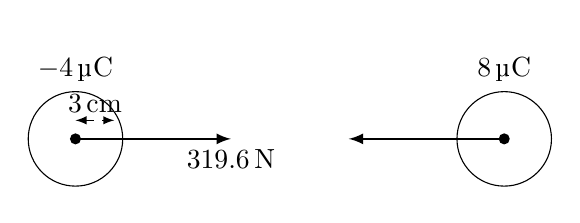
\begin{tikzpicture}
\begin{axis}[width=8cm,height=3.7cm,
    clip=false,
    xmin=-0.5,xmax=6,ymin=-0.6,ymax=1.2,
    axis line style={draw=none},
    ticks=none,    
]
    \fill (0,0) circle (2pt);
    \draw (0,0) circle (6mm) node[above=6mm] {$\SI{-4}{\micro C}$};
    \draw[->,thick] (0,0) -- ++(axis direction cs: 2,0) node[below] {$\SI{319.6}{N}$};

    \begin{scope}[xshift=5.5*0.99 cm]
        \fill (0,0) circle (2pt);
        \draw (0,0) circle (6mm) node[above=6mm] {$\SI{8}{\micro C}$};
        \draw[->,thick] (0,0) -- ++(axis direction cs: -2,0); % node[below] {$F$};
    \end{scope}

    \draw[<->,dashed] (0,0.2) -- ++(axis direction cs: 0.5,0);
    \node[above=6pt] at (0.5/2,0) {\SI{3}{cm}};
\end{axis}
\end{tikzpicture}
\end{center}

(a) If we \textit{triple} the distance between the charges and make the positive charge 45 times stronger, by what factor will the electrostatic force change from the original \SI{319.6}{N} force? (b) Calculate the magnitude of the new force.
\end{example}

Solution: (a) Distance $r$ increases by a factor of 3, and charge $q_2$ increases by a factor of 45. The new force will change by the following factor:

\begin{equation*}
    \frac{F'}{F} \sim \frac{k q_1 q_2}{r^2} \sim \frac{(1)(1)(45)}{(3)^2} = \frac{45}{9} = 5
\end{equation*}

(b) The new force has a magnitude of 

\begin{equation*}
    F' = 5 \times \SI{319.6}{N} = \SI{1598}{N}
\end{equation*}

Note that even though the charges got farther apart, the overall net force increased because the second charge became stronger.


\subsection*{\ref{MeMuHN} Exercises}

\begin{exercise} \label{WFMudS}
    By what factor does the electrostatic force between two charged spheres change if the distance between the spheres is tripled?
\end{exercise}

\begin{exercise} \label{t77ZZC}
    The electrostatic force between two separated charges is \SI{7.0}{N}. Calculate the magnitude of the new force when the charges are brought 3 times closer. 
\end{exercise}

\begin{exercise} \label{yCR62E}
    When two charged spheres are separated by 12 meters, the electrostatic force between them is \SI{4.2e-5}{N}. If the distance between the spheres quadruples and one of the spheres loses half its charge, what is the magnitude of the new force?
\end{exercise}

\begin{exercise} \label{y5ONvE}
    Consider the attractive force between the charges below:

\begin{center}
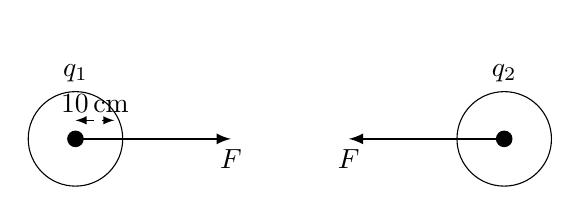
\begin{tikzpicture}
\begin{axis}[width=8cm,height=3.7cm,
    clip=false,
    xmin=-0.5,xmax=6,ymin=-0.6,ymax=1.2,
    axis line style={draw=none},
    ticks=none,    
]
    \fill (0,0) circle (3pt);
    \draw (0,0) circle (6mm) node[above=6mm] {$q_1$};
    \draw[->,thick] (0,0) -- ++(axis direction cs: 2,0) node[below] {$F$};

    \begin{scope}[xshift=5.5*0.99 cm]
        \fill (0,0) circle (3pt);
        \draw (0,0) circle (6mm) node[above=6mm] {$q_2$};
        \draw[->,thick] (0,0) -- ++(axis direction cs: -2,0) node[below] {$F$};
    \end{scope}

    \draw[<->,dashed] (0,0.2) -- ++(axis direction cs: 0.5,0);
    \node[above=6pt] at (0.5/2,0) {\SI{10}{cm}};
\end{axis}
\end{tikzpicture}
\end{center}

If the distance changes to \SI{84}{cm}, charge $q_1$ gets 15 times stronger, and $q_2$ gets 3 times weaker, by what factor does the electrostatic force change?
\end{exercise}



\begin{exercise} \label{sSztTO}
Consider the 99 nanocoulomb force between the charges below.

\begin{center}
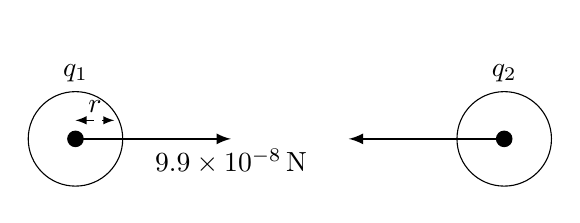
\begin{tikzpicture}
\begin{axis}[width=8cm,height=3.7cm,
    clip=false,
    xmin=-0.5,xmax=6,ymin=-0.6,ymax=1.2,
    axis line style={draw=none},
    ticks=none,    
]
    \fill (0,0) circle (3pt);
    \draw (0,0) circle (6mm) node[above=6mm] {$q_1$};
    \draw[->,thick] (0,0) -- ++(axis direction cs: 2,0) node[below] {$\SI{9.9e-8}{N}$};

    \begin{scope}[xshift=5.5*0.99 cm]
        \fill (0,0) circle (3pt);
        \draw (0,0) circle (6mm) node[above=6mm] {$q_2$};
        \draw[->,thick] (0,0) -- ++(axis direction cs: -2,0);
    \end{scope}

    \draw[<->,dashed] (0,0.2) -- ++(axis direction cs: 0.5,0);
    \node[above=6pt] at (0.5/2,0) {$r$};
\end{axis}
\end{tikzpicture}
\end{center}

(a) If $r$ decreases to one-sixth of its original value, $q_1$ gets 3 times stronger, and $q_2$ doubles in charge, by what factor does the electrostatic force change? (b) Calculate the new force.
\end{exercise}


\clearpage

\subsection{Answers to Select Exercises}


\ref{WFMudS}. $\frac{1}{9}$\\
\ref{t77ZZC}. \SI{63}{N}\\
\ref{yCR62E}. \SI{1.3e-6}{N}\\
\ref{y5ONvE}. 0.07\\
\ref{sSztTO}. (a) 216 \hspace{1em} (b) \SI{2.1e-5}{N}\\


\clearpage


\subsection{Ohm's Law} \label{nJeAQY}

Previously we defined \textbf{electric current} ($I$) as electric charge that moves through wires, and \textbf{resistance} ($R$) as the opposition of electric current by an element in a circuit. A third quantity is voltage.

\vspace{1em}

\textbf{voltage} ($V$) is defined as the electric potential energy per unit charge. You can think of voltage as the ``pressure or pushing force in a circuit\footnote{See ``\href{https://youtu.be/HsLLq6Rm5tU?t=291}{Ohms Law Explained}'' by The Engineering Mindset on \textit{YouTube}.}.'' It's supplied to a circuit by a battery. When current crosses an element with resistance, like a lamp or a resistor, voltage \textit{drops} across that element. Voltage is measured by connecting a voltmeter across circuit elements (batteries, resistors, etc.). The SI unit of voltage is the volt (V). 

\vspace{1em}

Next, we introduce Ohm's law, which links voltage, current, and resistance. \textbf{Ohm's law} states that electric current is proportional to the voltage applied across a circuit or other path. More usefully, Ohm's law in equation form is

\begin{equation} \label{cS0E6k}
    V = IR
\end{equation}

\begin{center}
    \begin{tabular}{cl|cc}
    \hline
    \textbf{Symbol} & \textbf{Quantity} & \textbf{SI Base Unit} & \textbf{Unit Symbol}  \\
    \hline\hline
    \rule{0pt}{2.5ex}
        $V$ & voltage & volt & V\\
        $I$ & current & ampere & A\\
        $R$ & resistance & ohm & \qty{}{\ohm}\\
    \hline
    \end{tabular}
\end{center}

\hrule

\begin{example}
    When a battery and 3.5-ohm resistor are connected in a circuit, the current through the wires is 0.43 amperes. What is the voltage of the battery?
\end{example}

Solution: It's good practice to draw a circuit diagram, to help you visualize the circuit:

\begin{center}
    \begin{circuitikz}
        \draw (0,2.5) to[battery,l_=$V$,i={$\SI{0.43}{A}$}] (0,0) -- (2,0) to[R,l_={$\SI{3.5}{\ohm}$}]
            (2,2.5) -- (0,2.5);
    \end{circuitikz}
\end{center}

We are given current and resistance through a series circuit: $I = \SI{0.43}{A}$ and $R = \qty{3.5}{\ohm}$. The unknown is the voltage: $V = \text{?}$ By Ohm's law (Eq.~\ref{cS0E6k}), the voltage supplied by the battery is

\begin{equation*}
    V = I R = (0.43)(3.5) = 1.5
\end{equation*}

Therefore, the battery's voltage is 1.5 volts.

\vspace{1em}

\hrule

\clearpage
\begin{example}
    What is the resistance of an automobile headlight through which \SI{2.50}{A} flows when \SI{12.0}{V} is applied to it?
\end{example}

Solution: We are given the current and voltage: $I = \SI{2.50}{A}$ and $V = \SI{12.0}{V}$. The unknown is the resistance: $R =\ ?$ These quantities are related by Ohm's law (Eq.~\ref{cS0E6k}):

\begin{equation*}
    V = IR
\end{equation*}

Substituting values leads to

\begin{equation*}
    12 = 2.5\,R
\end{equation*}

We solve for resistance as follows:

\begin{align*}
    \textbf{Write $R$ on left} \qquad & 2.5\,R = 12 \\[1ex]
    \textbf{Divide by 2.5} \qquad & \frac{\cancel{2.5}\,R}{\textcolor{red}{\cancel{2.5}}} = \frac{12}{\textcolor{red}{2.5}}\\[1ex]
    \textbf{Simplify} \qquad & R = \SI{4.8}{\ohm}
\end{align*}

The resistance in the headlight is 4.8 ohms.

\vspace{1em}

\hrule

\subsection*{\ref{nJeAQY} Exercises}

\setlength{\columnsep}{8mm}
\setlength{\columnseprule}{1pt}
\def\columnseprulecolor{\color{cyan}}

\begin{multicols*}{2}

\begin{exercise} \label{t0aM6F}
    Find the voltage of the battery in the circuit shown below.
\end{exercise}

\begin{center}
    \begin{circuitikz}
        \draw (0,2.5) to[battery,l_=$V$,i={$\SI{0.16}{A}$}] (0,0) -- (2,0) to[R,l_={$\SI{25}{\ohm}$}]
            (2,2.5) -- (0,2.5);
    \end{circuitikz}
\end{center}

\begin{exercise} \label{9ZzyyD}
    When a \qty{9.0}{V} battery and lamp are connected in a circuit, the resistance through the lamp is \qty{36}{\ohm}. What is the current through the lamp?
\end{exercise}

\begin{exercise} \label{x4zyhF}
    The current through a \SI{10}{\ohm} resistor 
    is \SI{0.25}{A}. What is the voltage drop across the resistor?
\end{exercise}

\begin{exercise}\label{CYRksH}
    Find the resistance of the unknown resistor shown below.
\end{exercise}

\begin{center}
    \begin{circuitikz}
        \draw (0,2.5) to[battery,l_=$\SI{4.5}{V}$,i={$\SI{0.9}{A}$}] (0,0) -- (2,0) to[R,l_={$R$}]
            (2,2.5) -- (0,2.5);
    \end{circuitikz}
\end{center}

\begin{exercise} \label{0rWTxi}
    What is the current through the lamp shown in the circuit below?
\end{exercise}

\begin{center}
    \begin{circuitikz}
        \draw (0,1.5) -- (0,0) to[lamp,l_=\qty{40}{\ohm}] (3,0) -- (3,1.5)
            to[battery,l_=\qty{8}{V},i=$I$] (0,1.5);
    \end{circuitikz}
\end{center}

\end{multicols*}


\clearpage
\subsection{Resistors in Series and Parallel} \label{TaE0On}

Consider two resistors in series or in parallel

\begin{center}
    \begin{circuitikz}
        \draw (0,0) to[R=$R_1$] (2.5,0) to[R=$R_2$] (5,0);
        \begin{scope}[xshift=7cm]
            \draw (0,0) -- (1,0) -- (1,1) to[R=$R_1$] (3,1) -- (3,0) -- (4,0)
                (1,0) -- (1,-1) to[R=$R_2$] (3,-1) -- (3,0);
        \end{scope}
    \end{circuitikz}
\end{center}

The equivalent resistance of resistors in series is

\begin{equation} \label{E2hx8w}
    R_{\mathrm{eq}} = R_1 + R_2
\end{equation}

For resistors in parallel, equivalent resistance is 

\begin{equation} \label{nxHaL8}
    R_{\mathrm{eq}} = \left(\frac{1}{R_1} + \frac{1}{R_2}\right)^{-1}
\end{equation}

\subsection*{\ref{TaE0On} Exercises}

\begin{multicols*}{2}
    


\begin{exercise} \label{z25jPn}
    \phantom{.}
    \begin{center}
        \tikz \draw (0,0) to[R=$\SI{17}{\ohm}$] (3,0) to[R=$\SI{71}{\ohm}$] (6,0);
    \end{center}
\end{exercise}

\begin{exercise} \label{NRON6F}
    \phantom{.}
    \begin{center}
        \tikz \draw (0,0) -- (1,0) -- (1,1) to[R=\SI{47}{\ohm}] (3,1) -- (3,0) -- (4,0)
        (1,0) -- (1,-1) to[R=\SI{75}{\ohm}] (3,-1) -- (3,0);
    \end{center}
\end{exercise}

\begin{exercise} \label{x7ZMs2}
    \phantom{.}
    \begin{center}
        \tikz \draw (0,0) to[R=\SI{22}{\ohm}] (3,0) to[R=\SI{56}{\ohm}] (6,0);
    \end{center}
\end{exercise}

\begin{exercise} \label{2QgW9g}
    \phantom{.}
    \begin{center}
        \tikz \draw (0,0) -- (1,0) -- (1,1) to[R=\SI{5}{\ohm}] (3,1) -- (3,0) -- (4,0)
        (1,0) -- (1,-1) to[R=\SI{86}{\ohm}] (3,-1) -- (3,0);
    \end{center}
\end{exercise}


\begin{exercise} \label{xjuTz7}
    \phantom{.}
    \begin{center}
        \tikz \draw (0,0) to[R=\SI{33}{\ohm}] (3,0) to[R=\SI{86}{\ohm}] (6,0);
    \end{center}
\end{exercise}

\begin{exercise} \label{MEfjff}
    \phantom{.}
    \begin{center}
        \tikz \draw (0,0) -- (1,0) -- (1,1) to[R=\SI{150}{\ohm}] (3,1) -- (3,0) -- (4,0)
        (1,0) -- (1,-1) to[R=\SI{101}{\ohm}] (3,-1) -- (3,0);
    \end{center}
\end{exercise}
\end{multicols*}

\clearpage

\subsection{Current in Series and Parallel} \label{GheYvY}

\begin{example} \label{0Jjx1M}
Go to the ``Circuit Construction Kit'' PhET (\href{https://phet.colorado.edu/sims/html/circuit-construction-kit-dc/latest/circuit-construction-kit-dc_en.html}{click here}). In PhET, build the following circuit, which contains two resistors in parallel. Use an ammeter to measure and record electric currents through all sections of wire. Using markers of different colors, highlight the entire section of wire if the current through that section is constant. Label the magnitude of current, in amperes, through each section.

\begin{center}
    \begin{circuitikz}
        \draw (3,4) -- (0,4) to[battery,l=\SI{12}{V}] (0,0) -- (3,0);
        \draw (3,4) to[R=\SI{3.0}{\ohm}] (3,0);
        \draw (3,4) -- (5,4) to[R=\SI{8.0}{\ohm}] (5,0) -- (3,0);
    \end{circuitikz}
\end{center}
\end{example}

Solution: When using the ammeter to measure current throughout different portions of wire, we see that there are 3 constant currents throughout the circuit: \SI{1.50}{A}, \SI{4.00}{A}, and \SI{5.50}{A}:

\vspace{1em}

\begin{minipage}{0.45\textwidth}
    \centering
    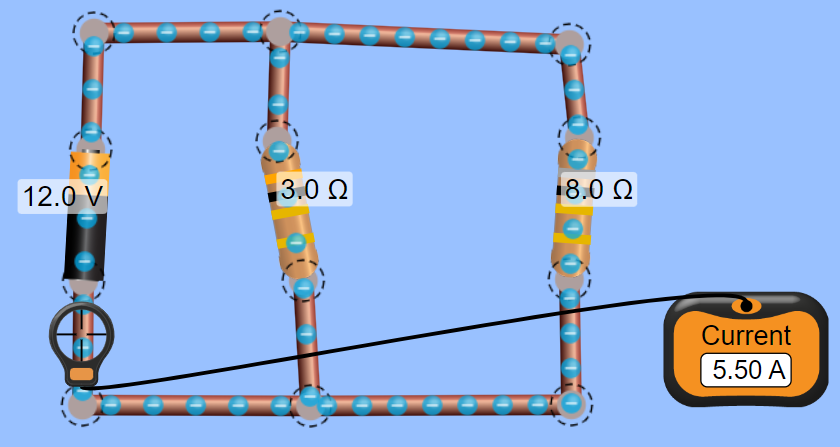
\includegraphics[width=7cm]{../figures/Unit9_PhET_Circuit2.png}
\end{minipage}%
\hspace{10mm}
\begin{minipage}{0.45\textwidth}
    \centering
    \begin{circuitikz}
        \draw[Green,thick] (3,0) -- (0,0) to[battery,color=Green,l=\SI{12}{V}, i=\SI{5.50}{A}] (0,4) -- (3,4);
        \draw[red,thick] (3,0) to[R,l_=\SI{3.0}{\ohm},color=red,i_=\SI{4.00}{A}] (3,4);
        \draw[blue,thick] (3,0) -- (5,0) to[R,l_=\SI{8.0}{\ohm},color=blue,i_=\SI{1.50}{A}] (5,4) -- (3,4);
    \end{circuitikz}
\end{minipage}

\vspace{1em}

\hrule

\begin{example}
    For the circuit in Example \ref{0Jjx1M}, use Ohm's law, in the \textit{absence} of an ammeter, to calculate the currents through each element.
\end{example}

Solution: Recall that Ohm's law relates voltage, current, and resistance as

\begin{equation*}
    V = I R
\end{equation*}

which implies that current is

\begin{equation*}
    I = \frac{V}{R}
\end{equation*}

In this circuit, the voltage drop across all components (battery and 2 resistors) is the voltage of the battery: 12 volts. The current through the first resistor is

\begin{equation*}
        I_1 = \frac{V}{R_1} = \frac{\SI{12}{V}}{\SI{3.0}{\ohm}} =  \SI{4.00}{A}
\end{equation*}

Current through the second resistor is

\begin{equation*}
    I_2 = \frac{V}{R_2} = \frac{\SI{12}{V}}{\SI{8.0}{\ohm}} = \SI{1.50}{A}
\end{equation*}

To find the current through the battery, we first need to calculate the equivalent resistance of the two resistors in parallel, using Equation \ref{nxHaL8}:

\begin{equation*}
    R_{\mathrm{eq}} = \left(\frac{1}{R_1} + \frac{1}{R_2}\right)^{-1} = \left(\frac{1}{3} + \frac{1}{8}\right)^{-1} = \SI{2.18}{\ohm}
\end{equation*}

Therefore, current through the battery is

\begin{equation*}
    I = \frac{V}{R_{\text{eq}}} = \frac{\SI{12}{V}}{\SI{2.18}{\ohm}} = \SI{5.50}{A}
\end{equation*}

\hrule

\subsection*{\ref{GheYvY} Exercises}

For each of the circuits below, calculate the three currents flowing through the wires. Draw a quick sketch, and label those currents on the sketch.

\begin{exercise} \label{Vr76KR}
    \phantom{.}
\end{exercise}

\begin{center}
    \begin{circuitikz}
        \draw (3,3) -- (0,3) to[battery,l=\SI{9}{V}] (0,0) -- (3,0);
        \draw (3,3) to[R=\SI{44}{\ohm}] (3,0);
        \draw (3,3) -- (5,3) to[R=\SI{77}{\ohm}] (5,0) -- (3,0);
    \end{circuitikz}
\end{center}

\begin{exercise} \label{wlE3QV}
    \phantom{.}
\end{exercise}

\begin{center}
    \begin{circuitikz}
        \draw (3,3) -- (0,3) to[battery,l=\SI{15}{V}] (0,0) -- (3,0);
        \draw (3,3) to[R=\SI{55}{\ohm}] (3,0);
        \draw (3,3) -- (5,3) to[R=\SI{80}{\ohm}] (5,0) -- (3,0);
    \end{circuitikz}
\end{center}

\begin{exercise} \label{XhaPdx}
    \phantom{.}
\end{exercise}

\begin{center}
    \begin{circuitikz}
        \draw (3,3) -- (0,3) to[battery,l=\SI{9}{V}] (0,0) -- (3,0);
        \draw (3,3) to[R=\SI{9.0}{\ohm}] (3,0);
        \draw (3,3) -- (5,3) to[R=\SI{37}{\ohm}] (5,0) -- (3,0);
    \end{circuitikz}
\end{center}








% \vspace{1em}

% \begin{circuitikz}
% \draw (0,3) to[battery, l=$V$,i=$I$] (0,0) -- (2,0)
% to[R=$R_2$] (2,3) -- (0,3);
% \draw (2,3) -- (4,3) to[R=$R_2$]
% (4,0) -- (2,0);
% \end{circuitikz}

% \begin{circuitikz}
% \draw (0,3) to[battery,l=$V$,i=$I$] (0,0);
% \draw (0,3) to[R=$R_1$] (3,3)
%     to[R=$R_2$] (3,0)
%     to[R=$R_3$] (0,0);
% \end{circuitikz}

\clearpage

\subsection{Voltage in Series and Parallel}

\begin{example}
    What is the voltage measured by the voltmeter across the resistor in the circuit below?

    \vspace{1em}
    
\begin{center}
\begin{circuitikz}
    \draw (0,0) -- (3,0) to[R=\SI{15}{\ohm}] ++(0,3) to[R=\SI{10}{\ohm}] ++(-3,0) to[battery,l=\SI{9.0}{V}] (0,0)
            (0.5,3) -- ++(0,1) to[rmeter,t=V] ++(2,0) -- ++(0,-1);
\end{circuitikz}
\end{center}

\end{example}

Solution:
To calculate the voltage through the 10-ohm resistor, we need to know the current through it. Since this circuit is in series, the same current runs through the whole circuit. This current is found be considering the equivalent resistance:

\begin{center}
\begin{circuitikz}
    \draw (0,0) -- (3,0) to[R,l_=$R_{\mathrm{eq}}$] ++(0,3) -- ++(-3,0) to[battery,l=\SI{9.0}{V}] (0,0)
            (0.5,3);
\end{circuitikz}
\end{center}

where equivalent resistance is, by Eq.~(\ref{E2hx8w}),

\begin{equation*}
    R_{\mathrm{eq}} = R_1 + R_2 = \SI{10}{\ohm} + \SI{15}{\ohm} = \SI{25}{\ohm}
\end{equation*}

The voltage of the battery is $V = \SI{9.0}{V}$, and the current through the circuit, by Ohm's law ($V = I R$), is

\begin{equation*}
    I = \frac{V}{R_{\text{eq}}} = \frac{\SI{9}{V}}{\SI{25}{\ohm}} = \SI{0.36}{A}
\end{equation*}

This 0.36-ampere current runs through the 10-ohm resistor, so the voltage across that resistor is

\begin{equation*}
    V = IR = (0.36)(10) = \SI{3.6}{V}
\end{equation*}

Therefore, the voltmeter reads 3.6 volts.

\vspace{1em}

\hrule

\clearpage

\subsection*{Exercises}

Calculate the voltage measured by the voltmeter in each of the circuits below.

\begin{exercise} \label{m9FFN5}
\phantom{.}

\begin{center}
\begin{circuitikz}
    \draw (0,0) -- (3,0) to[R=\SI{15}{\ohm}] ++(0,3) to[R=\SI{10}{\ohm}] ++(-3,0) to[battery,l=\SI{9.0}{V}] (0,0)
            (0.5,3);
    \draw (3,2.5) -- ++(1,0) to[rmeter,t=V] ++(0,-2) -- ++(-1,0);
\end{circuitikz}
\end{center}

\end{exercise}

\begin{exercise} \label{mLtImA}
\phantom{.}

\begin{center}
\begin{circuitikz}
    \draw (0,0) -- (3,0) to[R=\SI{25}{\ohm}] ++(0,3) to[R=\SI{75}{\ohm}] ++(-3,0) to[battery,l=\SI{60}{V}] (0,0)
            (0.5,3) -- ++(0,1) to[rmeter,t=V] ++(2,0) -- ++(0,-1);
\end{circuitikz}
\end{center}
\end{exercise}

\begin{exercise} \label{49hnUx}
\phantom{.}

\begin{center}
\begin{circuitikz}
    \draw (0,0) -- (3,0) to[R=\SI{18}{\ohm}] ++(0,3) to[R=\SI{24}{\ohm}] ++(-3,0) to[battery,l=\SI{15}{V}] (0,0)
            (0.5,3);
    \draw (3,2.5) -- ++(1,0) to[rmeter,t=V] ++(0,-2) -- ++(-1,0);
\end{circuitikz}
\end{center}

\end{exercise}



\clearpage
\subsection*{Answers to Select Exercises}

\ref{t0aM6F}. \SI{4.0}{V}\\
\ref{9ZzyyD}. \SI{0.25}{A}\\
\ref{x4zyhF}. \SI{2.5}{V}\\
\ref{CYRksH}. \SI{5.0}{\ohm}\\
\ref{0rWTxi}. \SI{0.2}{A}\\
\ref{z25jPn}. \SI{88}{\ohm}\\
\ref{NRON6F}. \SI{28.9}{\ohm}\\
\ref{x7ZMs2}. \SI{78}{\ohm}\\
\ref{2QgW9g}. \SI{4.72}{\ohm}\\
\ref{xjuTz7}. \SI{119}{\ohm}\\
\ref{MEfjff}. \SI{60.4}{\ohm}\\
\ref{Vr76KR}. \SI{0.20}{A}, \SI{0.11}{A}, \SI{0.32}{A}\\ 
\ref{wlE3QV}. \SI{0.27}{A}, \SI{0.19}{A}, \SI{0.46}{A}\\ 
\ref{XhaPdx}. \SI{1.0}{A}, \SI{0.24}{A}, \SI{1.24}{A}\\ 
\ref{m9FFN5}. \SI{5.4}{V}\\
\ref{mLtImA}. \SI{45}{V}\\
\ref{49hnUx}. \SI{6.4}{V}\\


% \clearpage
\subsection*{Additional Resources}

``Ohms Law Explained'' by \texttt{The Engineering Mindset} on \textit{YouTube} (\href{https://youtu.be/HsLLq6Rm5tU}{click here})

\textit{YouTube}: ``Resistors in Series and Parallel'' by \texttt{Ben Finio} 
(\href{https://youtu.be/bTnQUZ4Hi-E}{click here})

\clearpage


\end{document}

% \begin{tabular}{|m{0.25\textwidth}|m{0.7\textwidth}|}
%     \hline  
%     \cellcolor{black!20}\textbf{Date} &
%     \cellcolor{black!20}\textbf{Day 2023} \\
%     \hline
%     Learning Intention (TPO) &  \\
%     \hline
%     Hook/Warm Up/Opening & \\
%     \hline
%     Lesson/Learning Activities & \\
%     \hline
%     Graded Activities & \\
%     \hline
%     Closure & \\  
%     \hline
% \end{tabular}  

%%%%%%%%%%%%%%%%%%%%%%%%%%%%%%%%%%%%%%%%%%%%%%%%%%%%%%%%%

\begin{example}
    A rain cloud discharges 100 billion billion excess electrons through a lightning strike. What is the total charge carried by the lightning strike?
\end{example}

Solution: We are given the number of excess electrons:

\begin{equation*}
    n = \text{100 billion billion} = 100 \times 10^9 \times 10^9 = 100 \times 10^{18}
\end{equation*}

or simply just $10^{20}$ electrons. The charge on just \textit{one} electron is the negative elementary charge: $-e = \qty{-1.602e-19}{C}$. Therefore, the charge carried by the lightning is 100 billion billion times $-e$:

\begin{equation*}
    q = - n e = -(100 \times 10^{18}) \times \left(\qty{1.602e-19}{}\right) = \qty{-16}{C}
\end{equation*}